\chapter{Materialien und Methoden}
\label{cha:Materials}

\section{Wahl des Robotersystems}

Als Materialien stehen für das Projekt diverse Hardwaremodule zur Verfügung. Um die Problemstellung zu erfüllen ist zunächst ein mobiler Roboter notwendig. Für schnelle Prototypen-Erstellung bieten sich die Roboter-Baukästen von LEGO an.

\subsection{LEGO Mindstorms}

LEGO Mindstorms ist eine Produktreihe des Spielzeugherstellers LEGO, die bereits in drei Generationen erschienen ist. Sie zeichnen sich durch einen programmierbaren Hauptstein aus, der mit modularen Sensoren und Aktoren erweitert und in LEGO Technik-Aufbauten eingesetzt wird.

\subsubsection{LEGO Mindstorms NXT}

\begin{figure}[h]
\centering
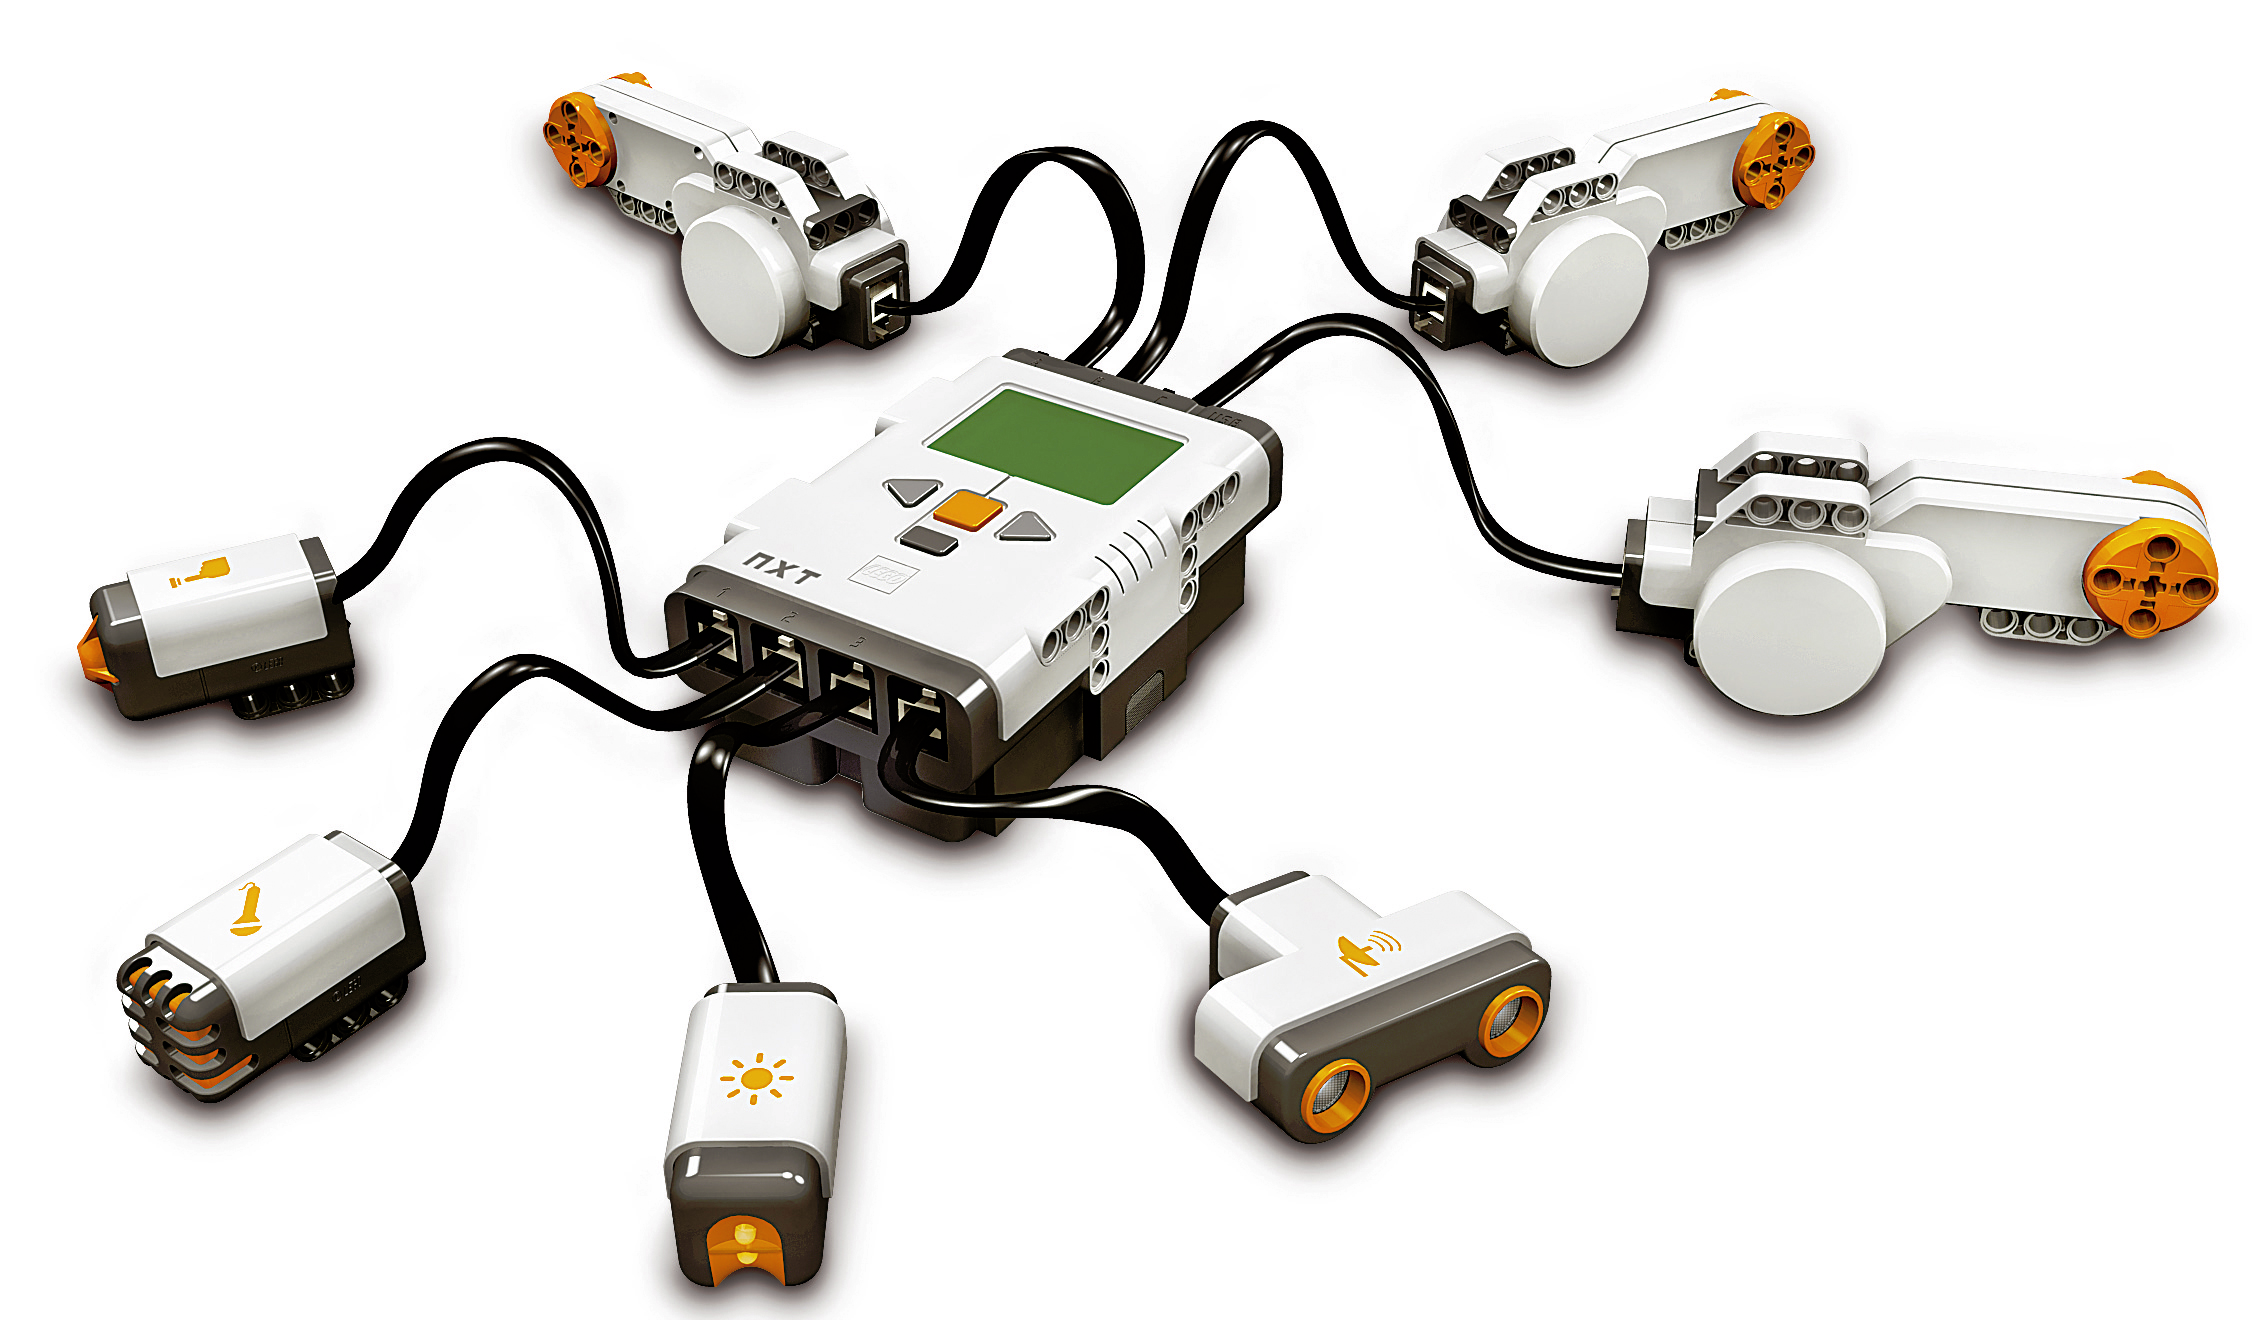
\includegraphics[width=0.8\textwidth]{Bilder/MatsAndMets/nxt}
\caption{Hauptbestandteile des LEGO Minstorms NXT-Systems}
\label{fig:nxt}
\end{figure}

Der NXT-Bausatz besteht wie alle Mindstorms-Reihen aus einem intelligenten Baustein als Recheneinheit und Kernstück des Roboters. Er beinhaltet einen 32-Bit ARM7-Prozessor (48 MHz) und einen 8-Bit Atmega-Mikrocontroller als Koprozessor zur Ausführung der über die USB-Schnittstelle übertragenen Programme.

Programmieren kann man den NXT über die von LEGO bereitgestellte graphische Entwicklungsumgebung NXT-G, was für Einsteiger den einfachsten Weg darstellt. Jedoch existieren auch für zahlreiche weitere Programmiersprachen wie C, Java, C\#, Matlab, Lua oder Ruby APIs zum Ansteuern der verschiedenen Funktionen.

An den Hauptstein können bis zu drei Motoren und bis zu vier Sensoren angeschlossen werden. Kommuniziert wird hierbei im I$^2$C-Protokoll. Die Servomotoren besitzen einen eingebauten Rotationssensor, die sich über den Rückkanal beim NXT-Stein melden.

Statusmeldungen werden über ein monochromes 100 mal 64 Pixel LCD-Display ausgegeben, auch bietet der Hauptstein einen eingebauten Lautsprecher und ein Bluetooth-Modul.

Als Sensoren sind eine große Auswahl von LEGO erhältlich:
\begin{itemize}
\item Tastsensor
\item Ultraschallsensor
\item Lichtsensor
\item Schallsensor
\item RFID-Sensor
\item Infrarot-Sensor
\item Beschleunigungssensor
\end{itemize}

Darüber hinaus können über Adapterkabel viele weitere Aktoren und Sensoren die das I$^2$-Protokoll beherrschen (unter anderem die des älteren RCX-Systems) angeschlossen werden, was fast keine Bedürfnisse beim Roboterbau offen lässt.

Das Gerüst bilden wie bei allen LEGO-Systemen die tausende verschiedenen Bauteile von LEGO Technik, was den NXT für fast jeden erdenklichen Einsatzbereich qualifiziert.

Die Datenblätter aller Komponenten und Protokolle sind frei von LEGO erhältlich, was NXT auch für Elektronik-Bastler interessant macht.

\subsubsection{LEGO Mindstorms EV3}

\begin{figure}[h]
\centering
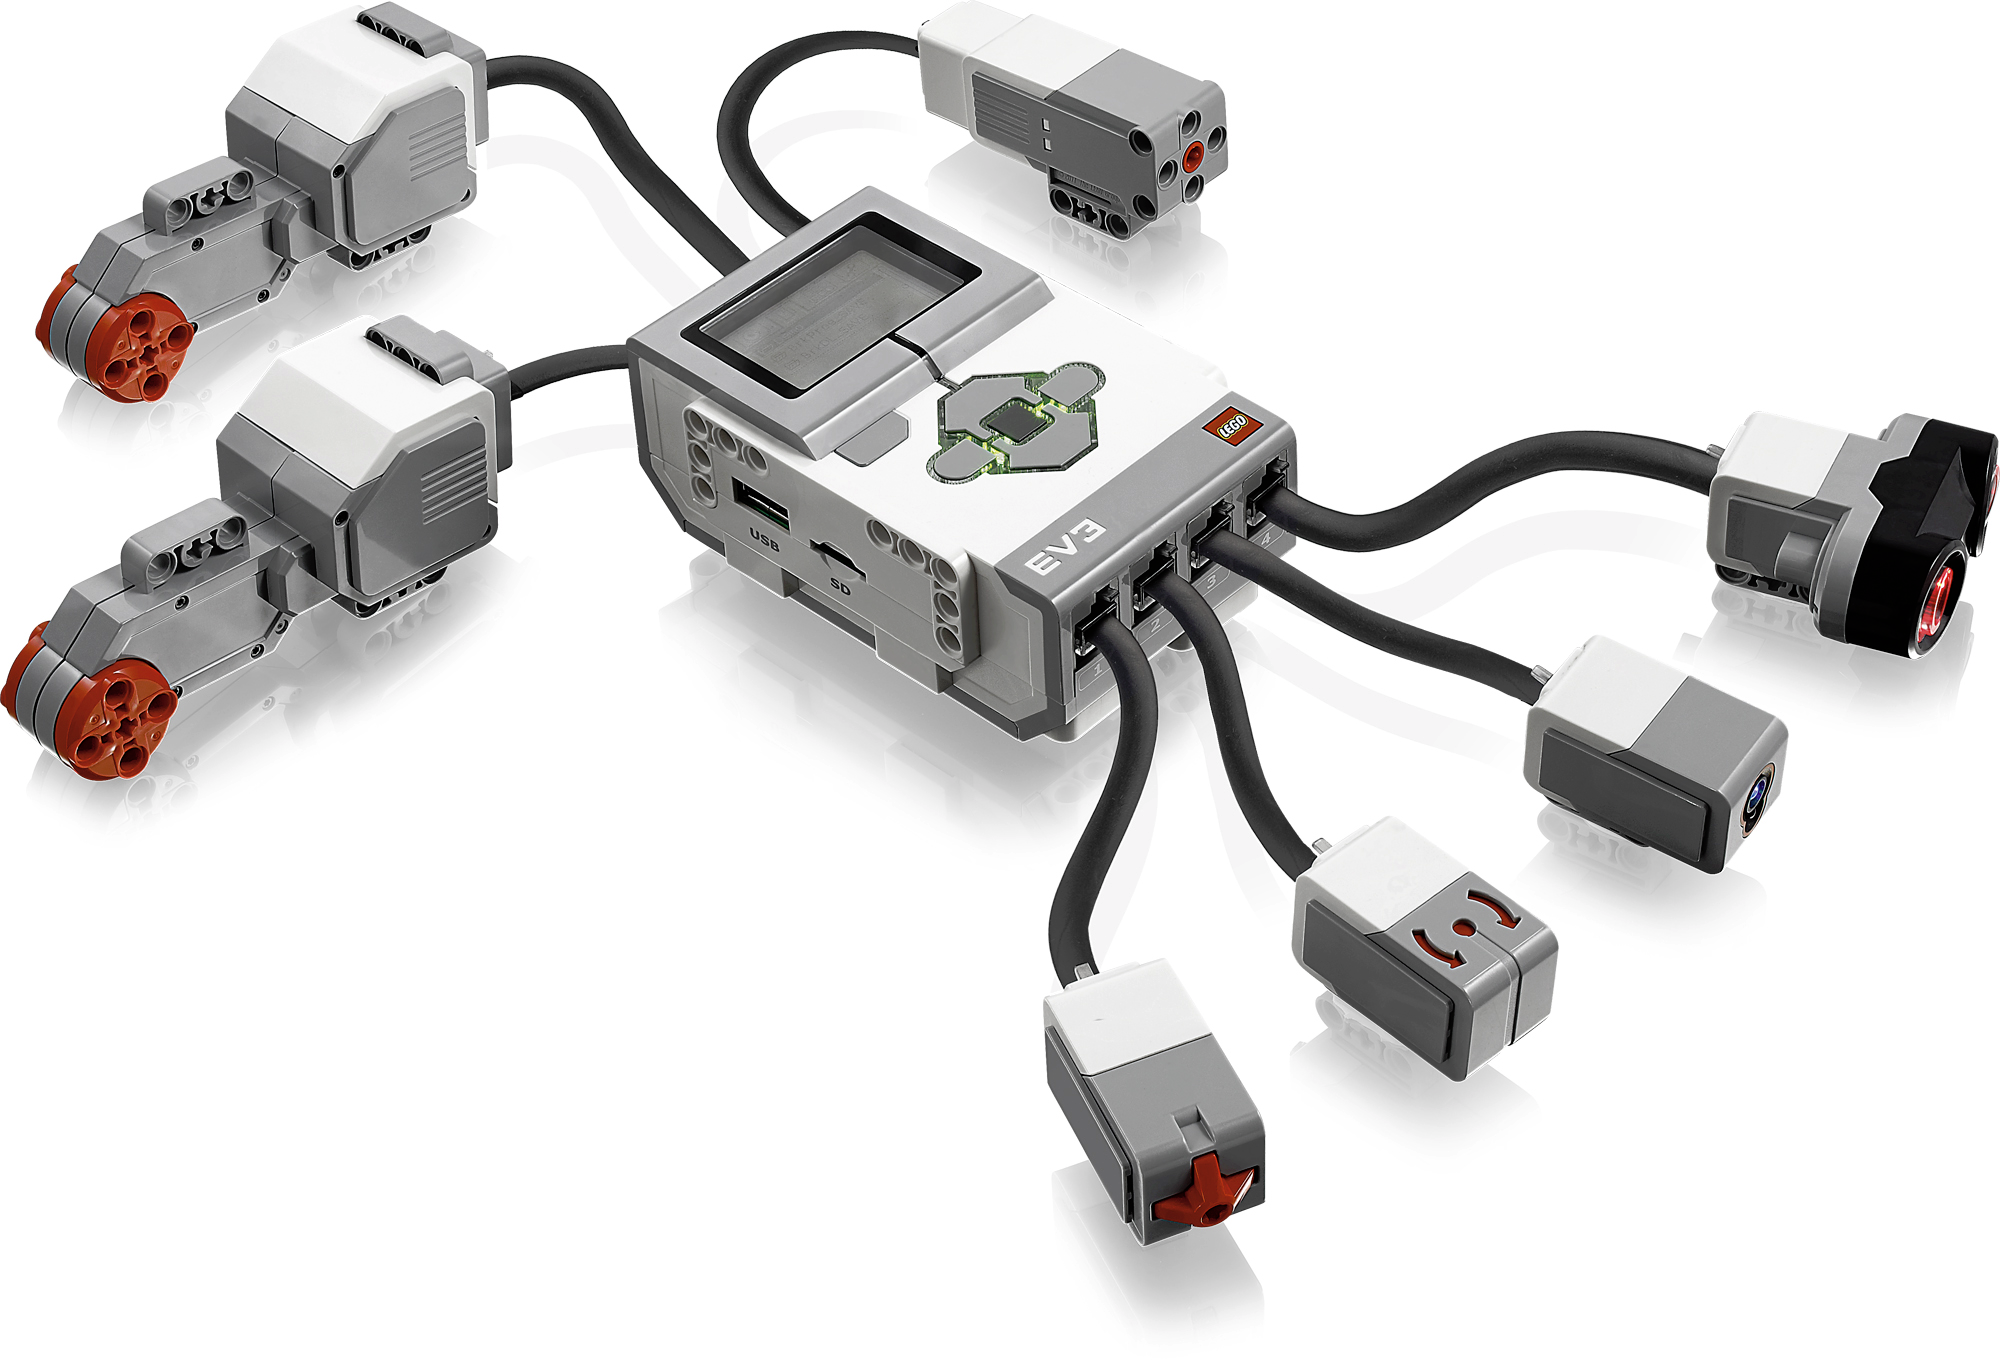
\includegraphics[width=0.8\textwidth]{Bilder/MatsAndMets/ev3}
\caption{Hauptbestandteile des LEGO Minstorms EV3-Systems}
\label{fig:ev3}
\end{figure}

EV3 stellt die Nachfolge-Kollektion von NXT dar. Die Hauptänderung besteht in Ersetzen des ARM7-Prozessor durch einen ARM9-Prozessor (300 MHz), auf dem eine Linuxumgebung ausgeführt wird. Eine Schnittstelle für microSD-Karten wurde hinzugefügt, welche als Programm- und Ressourcenspeicher dient.

EV3 ist kompatibel zu allen NXT-Sensoren und -Motoren und besitzt einen weiteren Ausgang am EV3-Stein. Das LCD-Display ist auf 178 mal 128 Pixel gewachsen. Das Design der Module wurde leicht geändert, die Auswahl ist bis auf ein weiteres, kleineres Motormodul identisch zu NXT.

Das Linux-Betriebssystem ermöglicht es im Vergleich zum Mikrocontroller des NXT, weit größere und komplexere Programme auszuführen und so den Aufgabenbereich zu erweitern. EV3 unterstützt offiziell die Verbindung zu Apple-Geräten.

Über einen neuen USB-Host-Anschluss können nun USB-Geräte wie ein optionales WLAN-Dongle angeschlossen werden, was die Erweiterungsmöglichkeiten vervielfacht.


\subsubsection{Fischertechnik Robotics}

\begin{figure}[h]
\centering
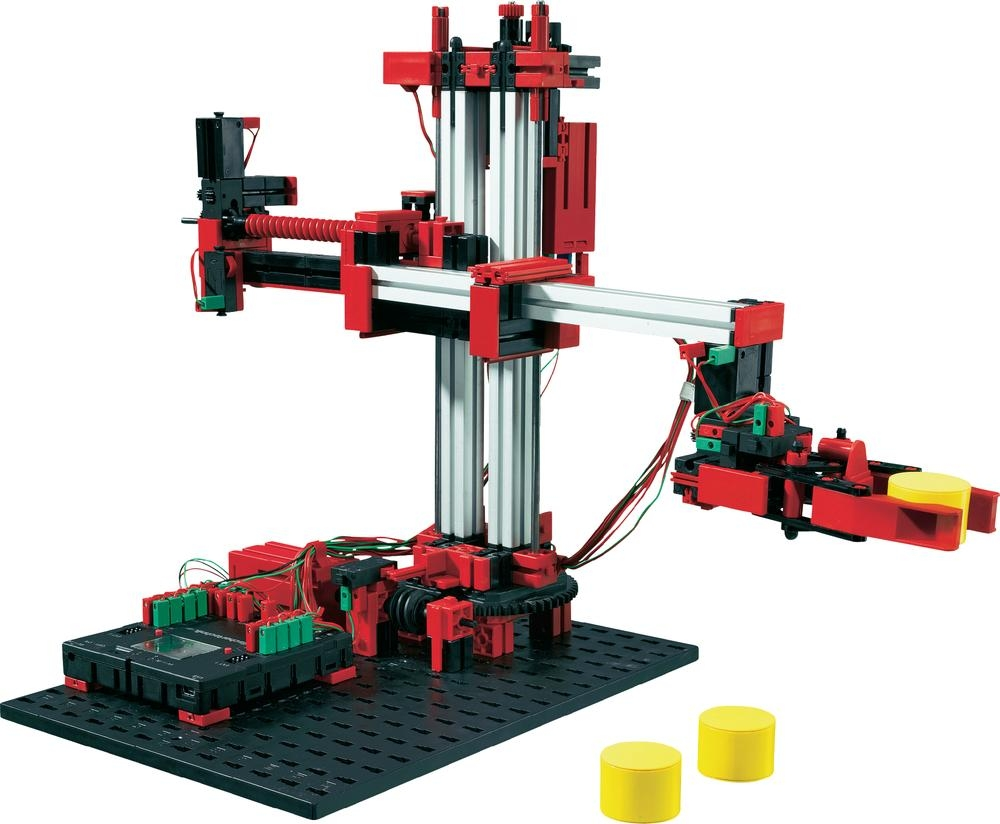
\includegraphics[width=0.8\textwidth]{Bilder/MatsAndMets/fischer}
\caption{Beispiel-Aufbau des Fischertechnik}
\label{fig:fischertechnik}
\end{figure}

Fischertechnik ist ein Konstruktions- und Baukastensystem, welches von den Fischerwerken produziert wird. Das Baukastensystem beruht auf einem Grundbaustein, der an allen 6 Seiten anbaubar ist. Für den Roboterbau stehen zusätzlich verschiedene Systemkomponenten wie Motoren, Zahnräder, Sensoren und Interfaces zur Verfügung. Diese sind sowohl untereinander als auch mit den Grundbausteinen beliebig kombinierbar.

Die Computing Bausätze als Grundaufbau eines Roboters sind sind in verschiedenen Varianten erhältlich und enthalten Bauanleitungen für drei bis acht Modelle. Sie sind mit unterschiedlichen Sensoren und Motoren ausgestattet, natürlich können auch hier selbst mit Bauteilen experimentiert und eigene Roboter entwickelt und gebaut werden.

Die Programmausführung übernimmt das ROBO Interface, aufbauend auf einen 16 Bit Mikrocontroller, vergleichbar mit den intelligenten Mindstorms-Steinen. Dieser wertet abhängig der Programmierung die Signale der Sensoren an den Eingängen aus und speist die Motoren an den Ausgängen.

An den PC angeschlossen wird das ROBO Interface entweder über ein 9-poliges serielles Kabel oder über USB. Funkübertragung zwischen PC und den Robotern wird durch das Erweiterungspack ROBO RF Data Link ermöglicht.

Mit bis zu drei Erweiterungsmodulen ROBO I/O-Extension stehen zusätzlich jeweils 4 weitere Motorenausgänge, 8 digitale und ein analoger Eingang zum Anschluss der Module zur Verfügung. Das IR Control Set erweitert das ROBO Interface um Fernsteuerung via Infrarot.

Programmiert wird wahlweise mithilfe der grafischen Programmieroberfläche ROBO Pro Software oder über freie APIs in den Sprachen C, C++, und Java.

\vspace{2em}

Letztendlich wurde sich für den LEGO Mindstorms NXT-Bausatz entschieden. Er bietet für den gedachten Einsatzzweck alle nötigen Module und Schnittstellen; Der Nachfolger EV3 wäre nur dann nötig, wenn auf dem Roboter komplexere Algorithmen abgearbeitet werden müssten, was den ARM7-Prozessor des NXT überfordern und die Linux-Umgebung des EV3 voraussetzen würde. Da hier jedoch sämtliche Berechnungen durch die App erledigt werden, ist dies nicht nötig.

Die Dokumentation der LEGO Mindstorms-Systeme sind wesentlich ergiebiger, frei erhältliche Anleitungen zahlreicher und der Einstieg wesentlich leichter als die des Sets von Fischertechnik Robotics, was einen Prototypen-Entwurf in Fischertechnik im Vergleich zu NXT verlängert hätte.

\section{Wahl des Kameramoduls}
\label{sec:Kamera}

Die Hauptfrage bezüglich des Kameramoduls bestand in der Wahl zwischen einem Ein- oder einem Zweikamerasystem.

Der Vorteil eines Zweikamerasystems besteht in der Möglichkeit für wesentlich bessere Orientierung im 3D-Raum, da Entfernungen mittels der beiden Differenzbilder präziser berechnet werden können.
Im Gegensatz dazu ist beim Einkamerasystem die Entfernungsberechnung auf ein 2D-Bild beschränkt und nicht annähernd so genau.

Jedoch ist der Berechnungsaufwand für das Auswerten zweier Differenzbilder ungleich höher, weshalb sich letztendlich aufgrund dieser Ungleichheit des Implementierungsaufwandes für ein Einkamerasystem entschieden werden.

Weitere Aspekte sind Auflösung und Öffnungswinkel des Kameramoduls.
Höhere Auflösung bedeutet bessere Erkennung von Gegenständen auf weitere Entfernungen; Ein größerer Öffnungswinkel heißt, dass mehr Raum in einem Bild erfasst werden kann, somit weniger Drehbewegung des Roboters in Richtung eines Objekts nötig ist, bis es erfasst und detektiert werden kann.

\begin{figure}[h]
\centering
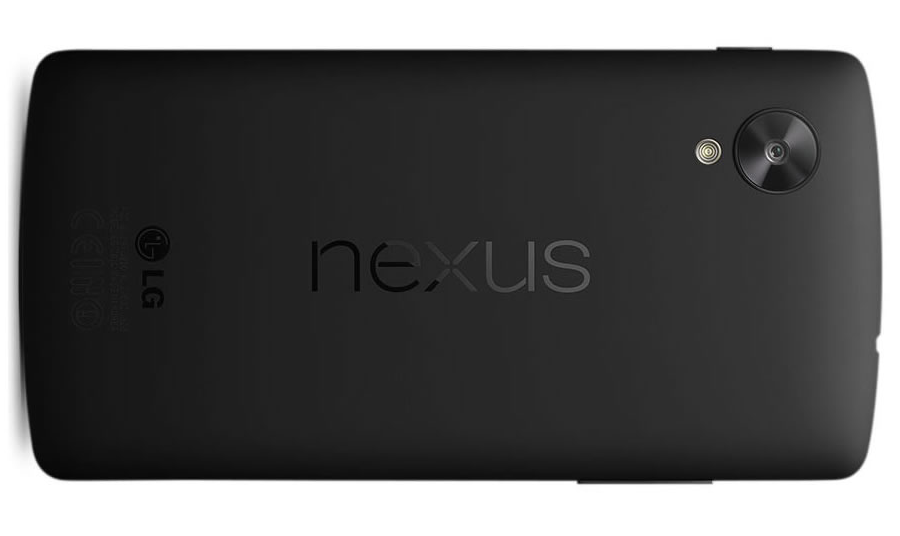
\includegraphics[width=0.5\textwidth]{Bilder/Robot/nexus_backside}
\caption{Kameramodul des Nexus 5}
\label{fig:camera}
\end{figure}

Ein Problem bei der Kamera des Nexus ist, das sich diese nicht zentral auf dem Rücken des Smartphones befindet, sondern nach links oben versetzt. Dies setzt voraus, dass entweder Software- oder Hardwareseitig dieser Versatz aus der Bildverarbeitung kompensiert wird.

Hier wurde der Einfachheit halber die Halterung am Roboter verschoben, wodurch aus der Sicht des Roboters die Kamera in der Mitte liegt.
